\documentclass{beamer}
\usepackage{animate}

\mode<presentation>
{
  \usetheme{Singapore}
  % or ...

  \setbeamercovered{transparent}
  % or whatever (possibly just delete it)
}

\usepackage[english]{babel}
\usepackage[latin1]{inputenc}
\usepackage{multirow}

%Beamer automatically puts the title up quite high where it appears
%over the background image of IARC: Keep adding empty lines until
%it appears in the right position
\title{~ \\ ~ \\ ~ \\ Everything You Ever Wanted to Know about Splines...}

\author{Martyn Plummer}
% - Use the \inst{?} command only if the authors have different
%   affiliation.

\institute[IARC] % (optional, but mostly needed)
{
  Infection and Cancer Epidemiology Group, IARC
}

\date[IARC]{15 June 2018}

%\newcommand{\thetavec}{\boldsymbol \theta}
%\newcommand{\Yvec}{\mathbf Y}

%Include IARC logo as background in slides
%\setbeamertemplate{background canvas}{\includegraphics
%        [width=\paperwidth,height=\paperheight]{logobg.jpg}}

\AtBeginSection[] % Do nothing for \section*
{
\begin{frame}<beamer>
\frametitle{Outline}
\tableofcontents[currentsection]
\end{frame}
}

\begin{document}

%{%Temporarily reset background for front page
%\setbeamertemplate{background canvas}{\includegraphics
%        [width=\paperwidth,height=\paperheight]{iarcbg.jpg}}
\begin{frame}[plain]
  \titlepage
\end{frame}
%}

\begin{frame}
  \frametitle{Overview}
  \tableofcontents
\end{frame}

\section{Categorization and its discontents}

\begin{frame}
  \frametitle{Rinaldi et al, JNCI. 2014 Jun;106(6):dju097}

  \begin{center}
  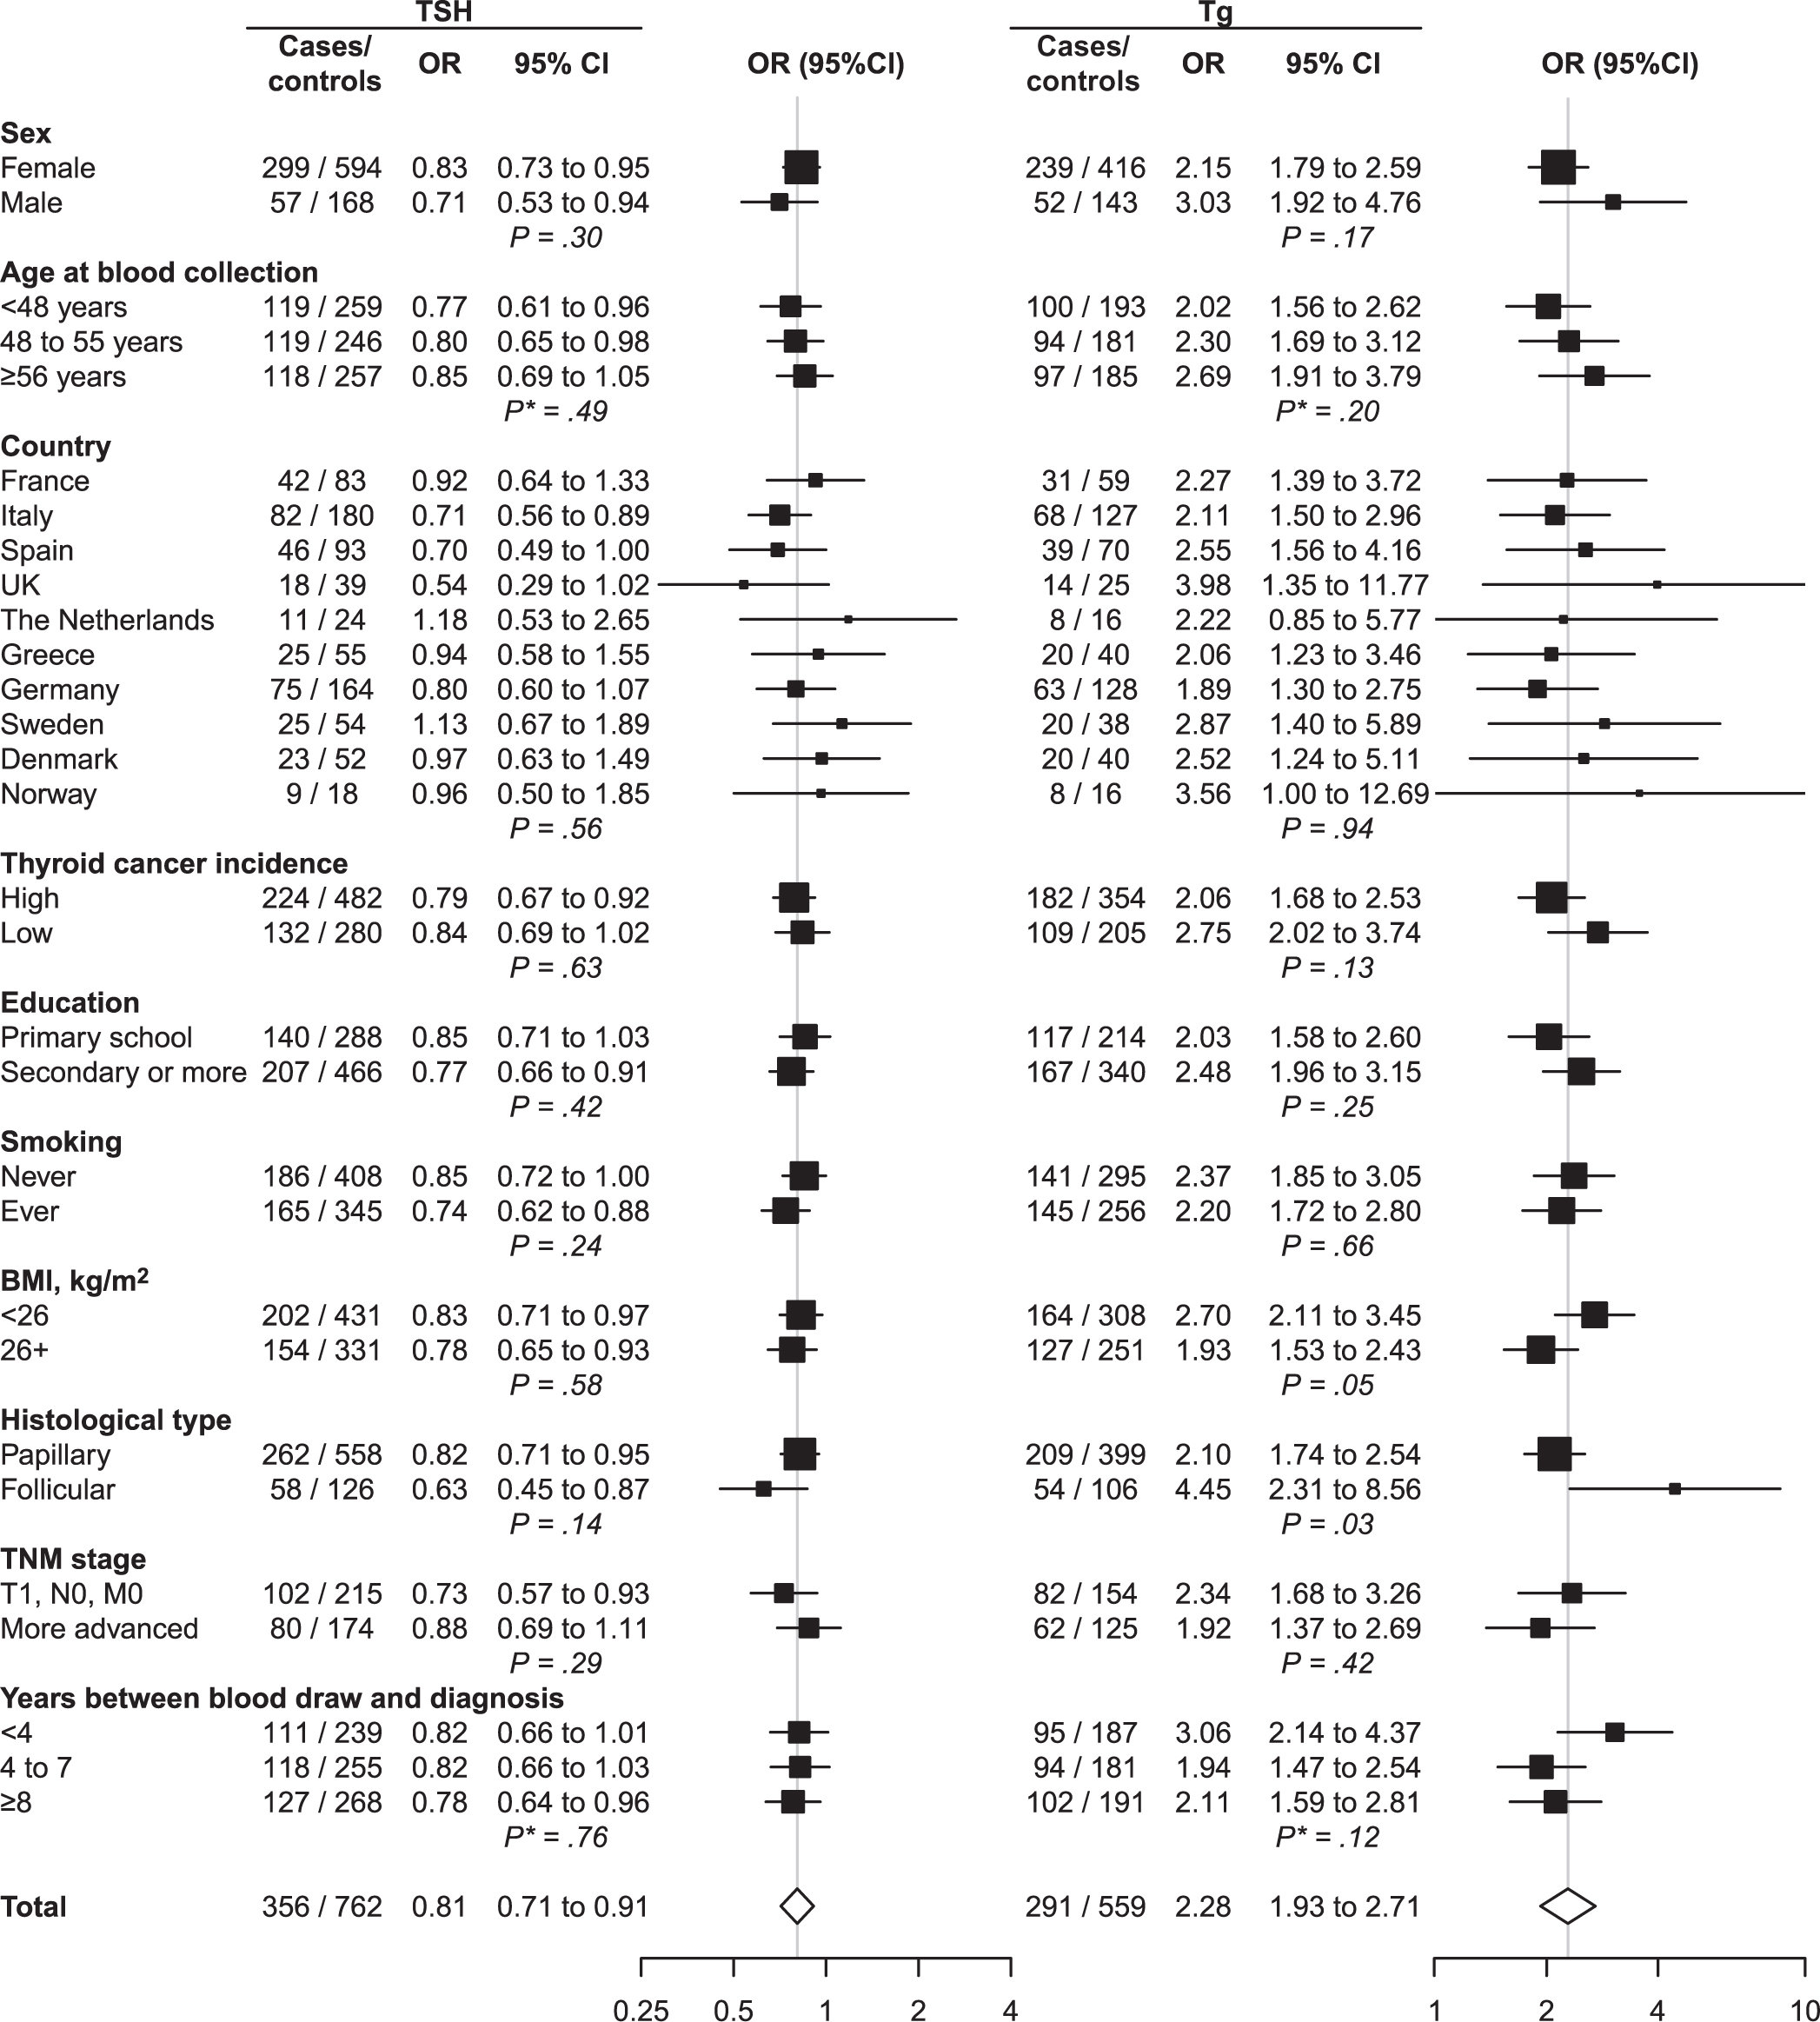
\includegraphics[scale=0.09]{figures/thyroid.png}
  \end{center}
  
\end{frame}

\begin{frame}
  \frametitle{Statisticians against categorization}
  \begin{itemize}
  \item Greenland S (1995) Avoiding power loss associated with
    categorization and ordinal scores in dose-response and trend
    analysis, Epidemiology, {\bf 6}, 450--454.
  \item Senn S (2005) Dichotomania: an obsessive compulsive disorder
    that is badly affecting the quality of analysis of pharmaceutical trials.
  \item Bennette C, and Vickers A, (2012), Against quantiles:
    categorization of continuous variables in epidemiologic research,
    and its discontents. BMC Medical Research Methodology 12:21
  \end{itemize}
\end{frame}

\begin{frame}
  \frametitle{Epidemiologists against categorization}

  Rose, G. (1992) The Strategy of Preventive Medicine
  \begin{itemize}
  \item Many diseases are not discrete. Instead there is an underlying
    continuum of increasing severity (e.g. hypertension).
  \item In medicine, we tend to conflate a clinical action (treat
    vs. do not treat) with the presence/absence of disease.
  \item Disease prevention efforts are best targeted at shifting the
    distribution of risk for the whole population instead of trying to
    identify and target a ``high risk'' group.
  \end{itemize}

\end{frame}
 
\section{Join the dots}

\begin{frame}
  \frametitle{Join the dots}

  \begin{center}
    \includegraphics<1>[scale=0.1]{figures/join-the-dots.png}
    \includegraphics<2>[scale=0.1]{figures/join-the-dots-solved.png}
  \end{center}
  
\end{frame}

\begin{frame}
  \frametitle{Linear interpolation}

  \begin{columns}
    \begin{column}{5cm}
      \includegraphics<1>[scale=0.4]{figures/dose-response-points.png}
      \includegraphics<2>[scale=0.4]{figures/dose-response-linear.png}
    \end{column}
    \begin{column}{4cm}
      \begin{itemize}
      \item Suppose a dose response curve is known exactly at certain
        points
      \item<2-> We can fill in the gaps (interpolate) by drawing a straight
        (linear) line between adjacent points
      \end{itemize}
    \end{column}
  \end{columns}
    
\end{frame}

\begin{frame}
  \frametitle{Why linear interpolation?}

  Out of all possible curves that go through the observed points,
  linear interpolation is the one that minimizes the penalty function
  \[
  \int \left( \frac{\partial f}{\partial x} \right)^2 dx
  \]

\end{frame}

\begin{frame}
  \frametitle{What does the penalty mean?}

  \begin{columns}
    \begin{column}{5cm}
      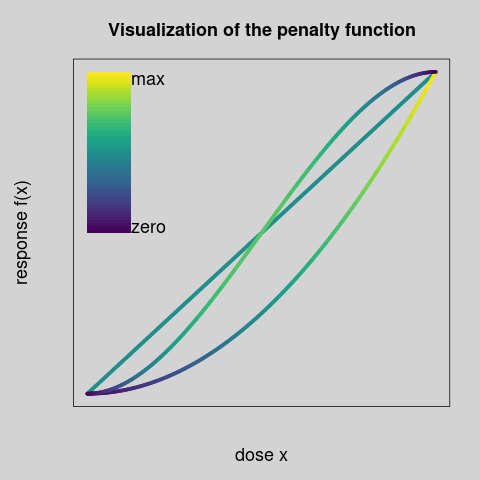
\includegraphics[scale=0.4]{figures/penalty1.png}
    \end{column}
    \begin{column}{4cm}
      \begin{itemize}
      \item The contribution to the penalty at each point depends on the
        steepness of the curve (represented by a colour gradient)
      \item  Any deviation from a straight line between the two fixed
        points will incur a higher penalty overall.
      \end{itemize}
    \end{column}
  \end{columns}
  
\end{frame}

\begin{frame}
  \frametitle{Extrapolation}

    \begin{columns}
    \begin{column}{5cm}
      \includegraphics<1>[scale=0.4]{figures/extrap1.png}
      \includegraphics<2>[scale=0.4]{figures/extrap2.png}
      \includegraphics<3>[scale=0.4]{figures/extrap3.png}
      \includegraphics<4>[scale=0.4]{figures/extrap4.png}
    \end{column}
    \begin{column}{4cm}
      \begin{itemize}
      \item Linear interpolation fits a linear dose-response curve exactly
      \item<3-> But it breaks down when we try to extrapolate
      \end{itemize}
    \end{column}
  \end{columns}

\end{frame}

\begin{frame}
  \frametitle{Why does linear interpolation break down?}

    \begin{itemize}
    \item The penalty function
      \[
      \int \left( \frac{\partial f}{\partial x} \right)^2 dx
      \]
      penalizes the steepness of the curve
    \item Minimizing the penalty function gives us gives us the ``flattest''
      curve that goes through the points.
      \begin{itemize}
      \item In between two observations the flattest curve is a
        straight line.
      \item Outside the range of the observations the flattest curve
        is completely flat.
      \end{itemize}
    \end{itemize}

\end{frame}

\begin{frame}
  \frametitle{A roughness penalty}

  \begin{itemize}
  \item If we want a fitted curve that extrapolates
    a linear trend then we want to minimize the \alert<2>{curvature}.
    \[
    \int \left(
    \frac{\partial\alert<2>{^2} f}{\partial x\alert<2>{^2}}
    \right)^2 dx
    \]
  \item Like the first penalty function but uses the \alert<2>{second
    derivative} of $f$ (i.e. the curvature).
  \item This is a roughness penalty.
  \end{itemize}
\end{frame}

\begin{frame}
  \frametitle{What does the roughness penalty mean?}

   \begin{columns}
    \begin{column}{5cm}
      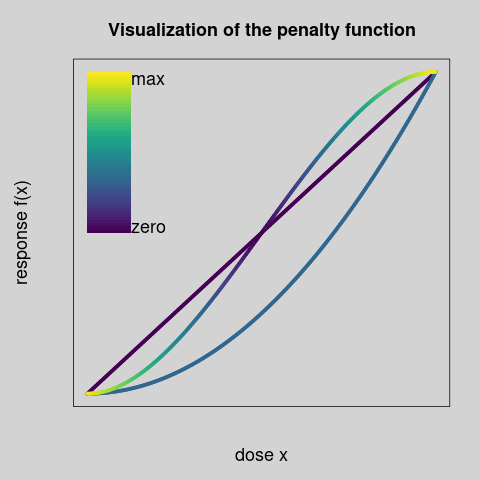
\includegraphics[scale=0.4]{figures/penalty2.png}
    \end{column}
    \begin{column}{4cm}
      \begin{itemize}
      \item The contribution to the penalty at each point depends on the
        curvature (represented by a colour gradient)
      \item A straight line has no curvature, hence zero penalty.
      \item Sharp changes in the slope are heavily penalized.
      \end{itemize}
    \end{column}
  \end{columns}

\end{frame}
    
\begin{frame}
  \frametitle{An interpolating cubic spline}

    \begin{columns}
    \begin{column}{5cm}
      \includegraphics<1>[scale=0.4]{figures/dose-response-points.png}
      \includegraphics<2>[scale=0.4]{figures/dose-response-cubic.png}
    \end{column}
    \begin{column}{4cm}
      \begin{itemize}
        \item The smoothest curve that goes through the observed
          points is a cubic spline.
      \end{itemize}
    \end{column}
  \end{columns}

\end{frame}

\begin{frame}
  \frametitle{Properties of cubic splines}

  \begin{itemize}
  \item A cubic spline consists of a sequence of curves of the form
    \[
    f(x) = a + b x + c x^2 + d x^3
    \]
    for some coefficients $a, b, c, d$, in between each observed point.
  \item The cubic curves are joined at the observed points (knots)
  \item The cubic curves match where they meet at the knots
    \begin{itemize}
    \item Same value $f(x)$
    \item Same slope $\partial f/ \partial x$
    \item Same curvature $\partial^2 f / \partial x^2$
    \end{itemize}
  \end{itemize}

\end{frame}

\section{Brownian motion}

\begin{frame}
  \frametitle{Brownian motion}

  \begin{columns}
    \begin{column}{5cm}
      \animategraphics[loop, controls,width=5cm]{12}{figures/bm/bm-}{0}{99}
    \end{column}
    \begin{column}{5cm}
      \begin{itemize}
        \item In 1827, botanist Robert Brown observed particles under
          the microscope moving randomly
        \item Theoretical explanation by Einstein (1905) in terms of
          water molecules
        \item Verified by Perrin (1908). Nobel prize in physics 1927.
      \end{itemize}
    \end{column}
    \end{columns}

\end{frame}

%%FIXME: Add something here about Wiener, Norbert
\begin{frame}
  \frametitle{Evolution of 1-dimensional Brownian motion with time}

  \begin{columns}
    \begin{column}{5cm}
      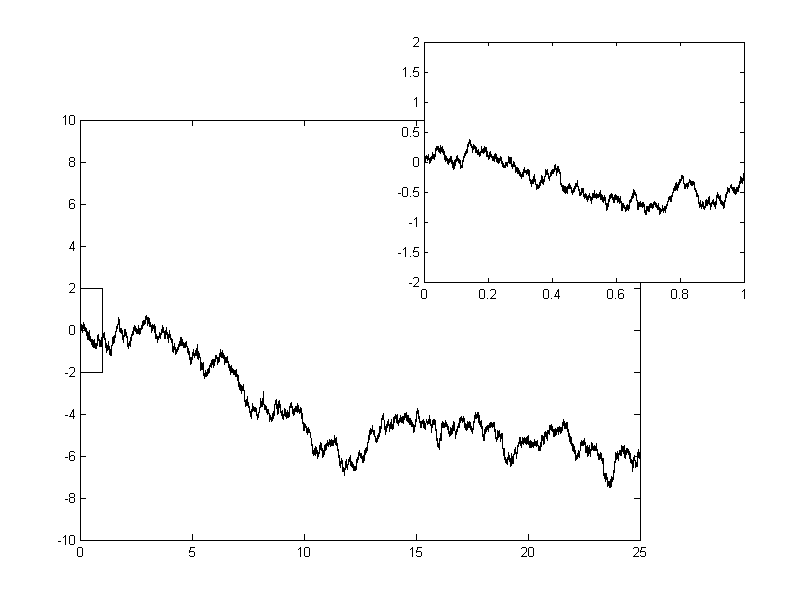
\includegraphics[scale=0.3]{figures/Wiener_process_zoom.png}
    \end{column}
    \begin{column}{5cm}
      \begin{itemize}
      \item In mathematics a Brownian motion is a stochastic process
        that randomly goes up or down at any time point
      \item Also called a Wiener process after American mathematician
        Norbert Wiener.
      \item A Brownian motion is fractal -- it looks the same if you
        zoom in and rescale
      \end{itemize}
    \end{column}
  \end{columns}
  
\end{frame}


\begin{frame}
  \frametitle{A partially observed Brownian motion}

  \begin{columns}
    \begin{column}{5cm}
      \includegraphics<1>[scale=0.4]{figures/linear1.png}
      \includegraphics<2>[scale=0.4]{figures/linear2.png}
      \includegraphics<3>[scale=0.4]{figures/linear3.png}
    \end{column}
    \begin{column}{4cm}
      \begin{itemize}
      \item Suppose we observe a Brownian motion at three points
      \item<2-> Grey lines show a sample of possible paths through the points
      \item<3-> The black line shows the average over all paths
      \end{itemize}
    \end{column}
  \end{columns}
    
\end{frame}

\begin{frame}
  \frametitle{Statistical model for linear interpolation}

  \begin{itemize}
  \item Suppose the curve $f$ is generated by the underlying model
    \[
    f(x) = \alpha + \sigma W(x)
    \]
    where $W$ (for Wiener process) is a Brownian motion
  \item Then given points $(x_1, f(x_1)) \ldots (x_n, f(x_n))$ the
    {\em expected value} of $f$ is the curve we get from linear
    interpolation.
  \end{itemize}
  
\end{frame}

\begin{frame}
  \frametitle{Integrated Brownian motion}

  \begin{columns}
    \begin{column}{5cm}
      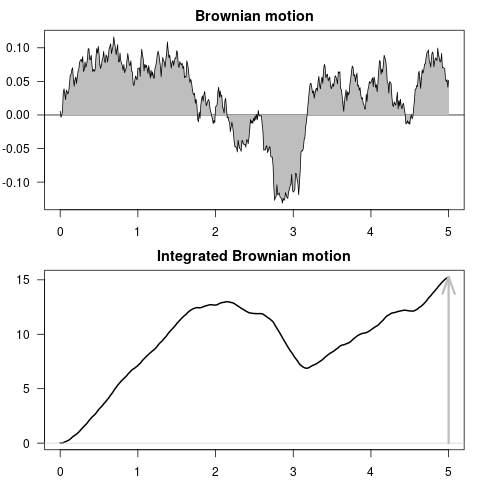
\includegraphics[scale=0.4]{figures/integrated.png}
    \end{column}
    \begin{column}{4cm}
      \begin{itemize}
      \item The value of an integrated Brownian motion is the area
        under the curve (AUC) of a Brownian motion up to that point.
      \item AUC goes down when the Brownian motion takes a negative
        value.
      \end{itemize}
    \end{column}
  \end{columns}

\end{frame}

\begin{frame}
  \frametitle{Integrated Brownian motion with drift}

  Add a mean parameter and a linear trend (drift) to the
  integrated Brownian motion:
  \[
  f(x) = \alpha + \beta x + \sigma \int_{0}^x W(z) dz
  \]
  This more complex model is capable of modelling smooth curves.

\end{frame}

\begin{frame}
  \frametitle{A partially observed integrated Brownian motion with drift}

  \begin{columns}
    \begin{column}{5cm}
      \includegraphics<1>[scale=0.4]{figures/cubic1.png}
    \end{column}
    \begin{column}{4cm}
      \begin{itemize}
      \item Grey lines show a sample of possible paths through the points
      \item The black line shows the average over all paths
      \end{itemize}
    \end{column}
  \end{columns}
    
\end{frame}

\begin{frame}
  \frametitle{Zoom on the expected value}

  \begin{columns}
    \begin{column}{5cm}
      \includegraphics<1>[scale=0.4]{figures/cubic2.png}
    \end{column}
    \begin{column}{4cm}
      \begin{itemize}
      \item The expected value is a cubic spline.
      \item Extrapolation beyond the boundary of the points is linear
        (natural spline).
      \end{itemize}
    \end{column}
  \end{columns}
    
\end{frame}

\begin{frame}
  \frametitle{The smoothness paradox}

  \begin{itemize}
  \item A cubic natural spline is the smoothest curve that goes through
    a set of points.
  \item But the underlying random process $f(x)$ is nowhere smooth.
  \item $f(x)$ is constantly changing its slope based on the value of the
    underlying Brownian motion.
  \end{itemize}
 
\end{frame}

\begin{frame}
  \frametitle{The knot paradox}

  \begin{itemize}
  \item There are no knots in the underlying model for a cubic natural
    spline.
  \item Knots are a result of the observation process.
  \end{itemize}

\end{frame}
  
\section{Smoothing splines}

\begin{frame}
  \frametitle{Dose response with error}

    \begin{columns}
    \begin{column}{6cm}
      \includegraphics<1>[scale=0.4]{figures/smooth1.png}
      \includegraphics<2>[scale=0.4]{figures/smooth2.png}
    \end{column}
    \begin{column}{4cm}
      In practice we never know the dose response curve exactly at any
      point but always measure with error. A spline model is then
      a compromise between
      \begin{itemize}
      \item Model fit
      \item Smoothness of the spline
      \end{itemize}
    \end{column}
    \end{columns}
    
\end{frame}

\begin{frame}
  \frametitle{Fitting a smoothing spline}

  Minimize
  \[
  \sum_i \left( y_i - f(x_i) \right)^2 + \lambda
  \int \left(
  \frac{\partial^2 f}{\partial x^2}
  \right)^2 dx
  \]
  Or, more generally
  \[
  \text{Deviance } + \lambda * \text{Roughness penalty}
  \]
  Size of tuning parameter $\lambda$ determines compromise between model fit
  (small $\lambda$) and smoothness (large $\lambda$).

\end{frame}

\begin{frame}
  \frametitle{How to choose the tuning parameter $\lambda$}

  This is a statistical problem. There are various statistical
  approaches:
  \begin{itemize}
  \item Restricted maximum likelihood (REML)
  \item Cross-validation
  \item Bayesian approach (with prior on smoothness)
  \end{itemize}
  At least the first two should be available in most software.
  
\end{frame}

\section{Conclusions}

\begin{frame}
  \frametitle{Spline models done badly}

  \begin{columns}
    \begin{column}{5cm}
      \begin{itemize}
      \item Choose number and placement of knots
      \item Create a spline bases
      \item Use spline basis as the design matrix in a generalized linear model.
      \end{itemize}
    \end{column}
    \begin{column}{5cm}
      \begin{itemize}
      \item Without penalization, model will underfit (too few knots)
        or overfit (too many knots)
      \item Placement of knots may create artefacts in the dose-response
        relationship
      \end{itemize}
    \end{column}
  \end{columns}

\end{frame}

\begin{frame}
  \frametitle{Spline models done well}

  \begin{columns}
    \begin{column}{5cm}
      \begin{itemize}
      \item A knot for every observed value (remember: knots are a
        product of the observation process).
      \item Use penalization: find the right compromise between model fit
        and model complexity.
      \end{itemize}
    \end{column}
    \begin{column}{5cm}
      \begin{itemize}
      \item In practice we can get a good approximation to this ``ideal''
        model with fewer knots.
      \item This assumption should be tested
      \end{itemize}
    \end{column}
  \end{columns}

\end{frame}

\begin{frame}
  \frametitle{Spline models in R}

  \begin{itemize}
  \item Do not use the \textsf{splines} package.
  \item Use the \texttt{gam} function from the \textsf{mgcv}
    package to fit your spline models.
  \item The \texttt{gam} function chooses number and placement of knots
    for you and estimates the size of the tuning parameter $\lambda$
    automatically.
  \item You can use the \texttt{gam.check} function to see if you have
    enough knots. Also re-fit the model explicitly setting a larger
    number of knots (e.g. double) to see if the fit changes.
  \end{itemize}

\end{frame}

\begin{frame}
  \frametitle{Penalized spline}

  \begin{columns}
    \begin{column}{6cm}
      \includegraphics<1>[scale=0.4]{figures/gam-points.png}
      \includegraphics<2>[scale=0.4]{figures/gam-7.png}
    \end{column}
    \begin{column}{4cm}
      \begin{itemize}
      \item A gam fit to some simulated data
      \item Model has 9 degrees of freedom
      \item Smoothing reduces this to 2.88 effective degrees of freedom
      \end{itemize}
    \end{column}
  \end{columns}
  
\end{frame}


\begin{frame}
  \frametitle{Unpenalized spline}

  \begin{columns}
    \begin{column}{6cm}
      \includegraphics<1>[scale=0.4]{figures/gam-points.png}
      \includegraphics<2>[scale=0.4]{figures/gam-nonsmoothed.png}
    \end{column}
    \begin{column}{4cm}
      \begin{itemize}
      \item An unpenalized spline using the same spline basis as the
        gam fit.
      \item Model has 9 degrees of freedom
      \end{itemize}
    \end{column}
  \end{columns}
  
\end{frame}

\end{document}
